\documentclass{article}

\usepackage{graphicx}

\begin{document}

\section{Logic Gates}
Logic gates perform logical operations that take binary input (0s and 1s) and produce a single binary output. They are used in most electronic device including:

\begin{table}[h!]
	\begin{center}
		\caption{Logic Gates}
		\label{tab:table1}
		\begin{tabular}{|l|c|c|}
			\hline
			Smartphones
			&
			Tablets
			&
			Memory Devices
			\\
		   \hline
		   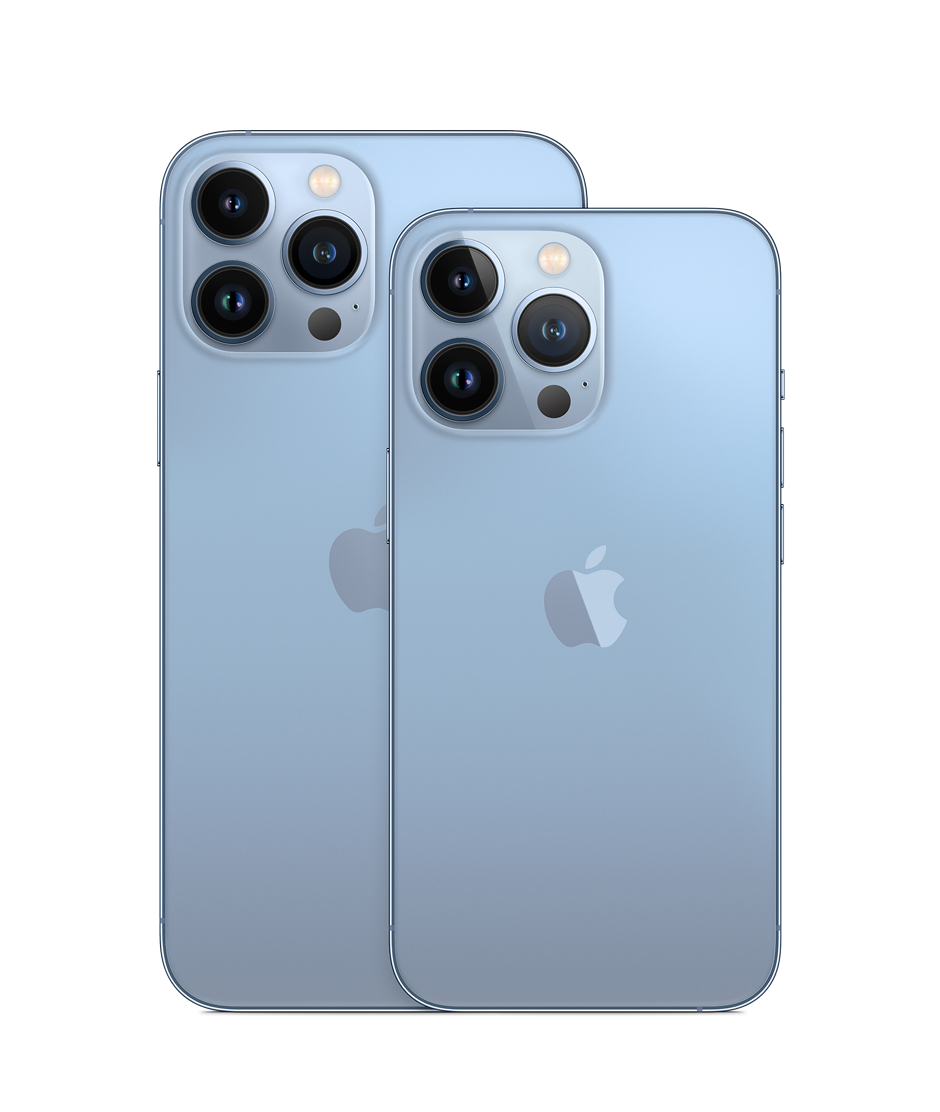
\includegraphics[width=0.2\linewidth]{Picture2}
		   &
		   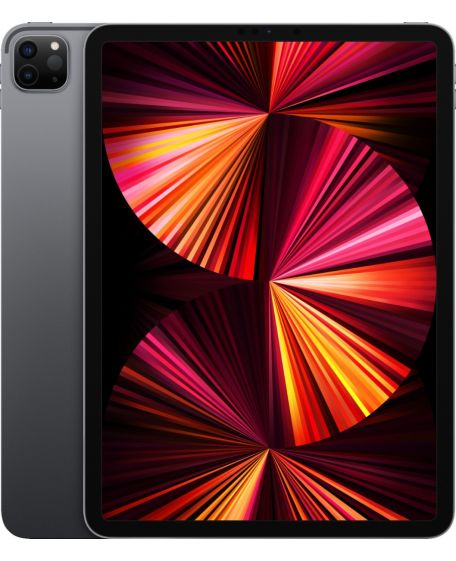
\includegraphics[width=0.2\linewidth]{Picture3}
		   &
		   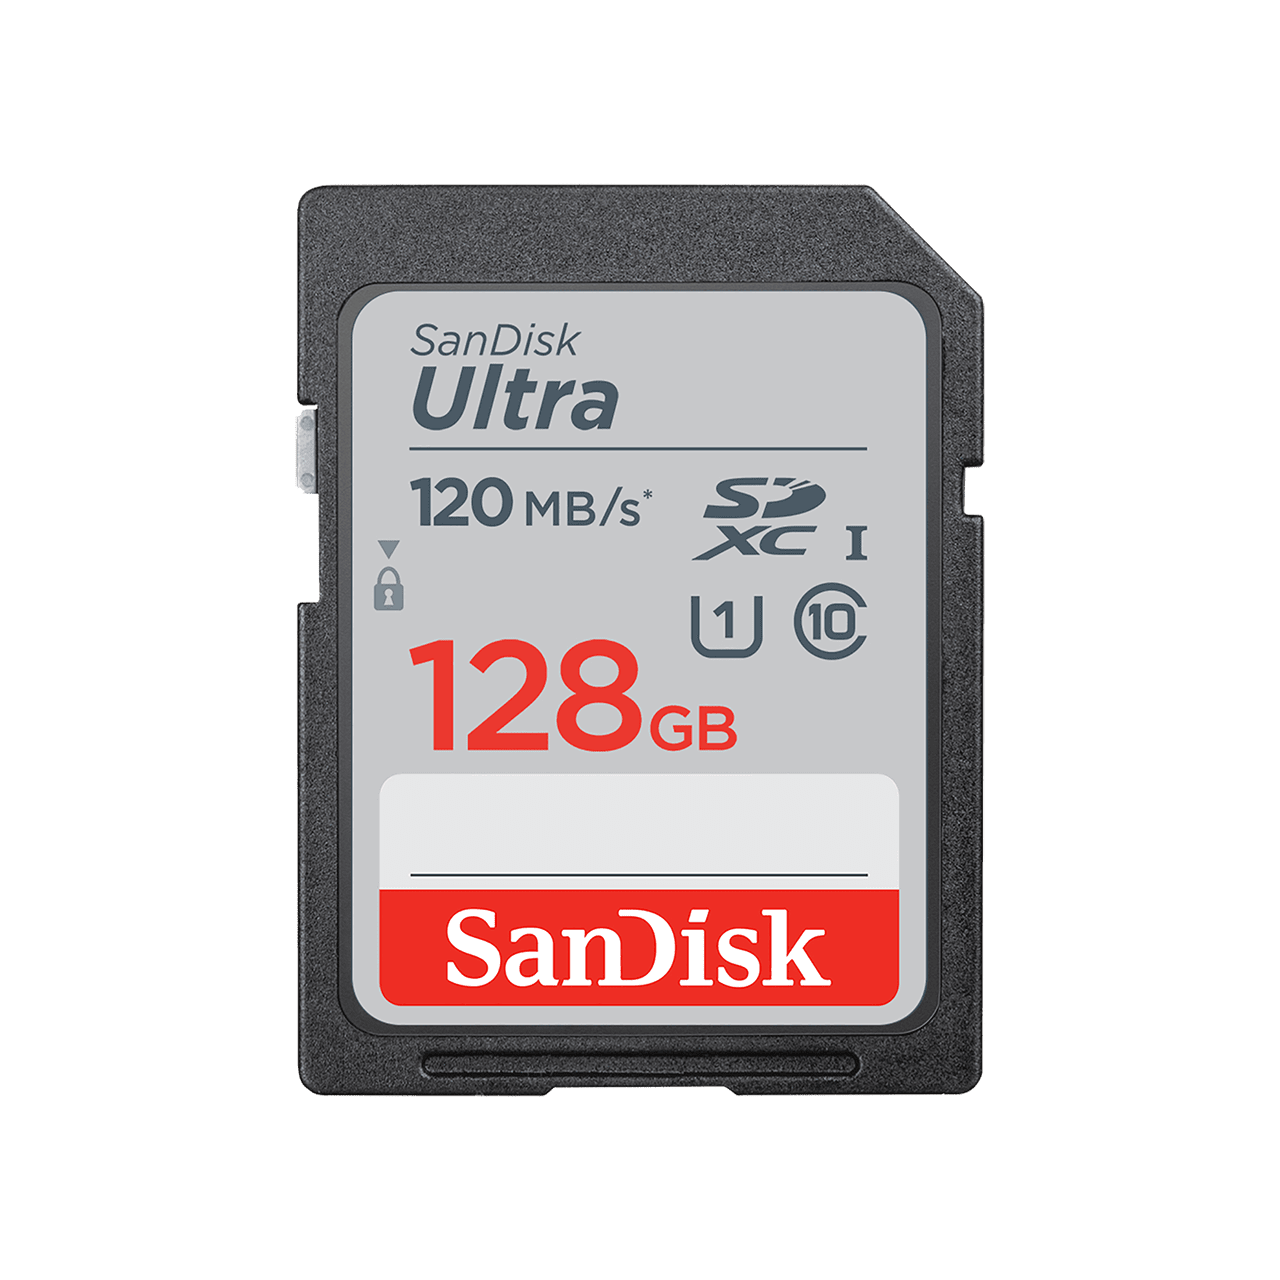
\includegraphics[width=0.2\linewidth]{Picture4}
		   \\
		     \hline
	     \end{tabular}     	
	\end{center}
\end{table}

\end{document}


\end{document}